\documentclass[conference]{IEEEtran}
\IEEEoverridecommandlockouts

\usepackage{amsmath,amssymb,amsfonts}
\usepackage{graphicx}
\usepackage{booktabs}
\usepackage{siunitx}
\usepackage{optidef}
\usepackage{tikz}
\usetikzlibrary{positioning,arrows.meta,calc}
\usepackage{xcolor}
\usepackage[hidelinks]{hyperref}

% words in subscripts are upright (\mathrm); one-letter variables stay italic.
\newcommand{\wvec}{w}
\newcommand{\Lmax}{L}
\newcommand{\Bmax}{B}
\newcommand{\wdcoef}{w_{\mathrm{d}}}
\newcommand{\yhat}{\hat{y}}
\newcommand{\Uc}{U(\wvec)}
\newcommand{\norm}[1]{\lVert #1 \rVert}
\DeclareMathOperator{\Lip}{Lip}

\begin{document}

\title{Neural Network Optimization\\
as a Constrained Nonlinear Program}

\author{\IEEEauthorblockN{Arindam Paul}
\IEEEauthorblockA{Numerical Optimization Project\\
Albert-Ludwigs-Universit\"at Freiburg, Summer Term 2026}}

\maketitle

\begin{abstract}
I study small neural-network regression written as a constrained nonlinear program
(NLP): the network weights are the decision variables, the mean-squared error is the
objective, and two requirements are imposed as hard constraints, a bound on the
network's input Lipschitz behaviour and a Euclidean norm ball on the weights. The
true Lipschitz constant is not directly convenient for the solver, so I enforce a
computable certificate $\Uc=\norm{\wvec_1}_2\norm{\wvec_2}_2$, a guaranteed upper
bound whose constraint $\Uc\le\Lmax$ is a conservative sufficient condition for an
$\Lmax$-Lipschitz map. I build the program in CasADi and solve it with the
interior-point solver IPOPT, comparing against matched soft-penalty Adam training on
the same requirements. IPOPT satisfies both constraints to solver tolerance in every
trial, while weight decay leaves the certificate uncontrolled; a converged
single-constraint penalty shows a feasibility transition near the associated
multiplier. Enlarging the network in width or depth yields no accuracy gain but
makes the interior-point solve markedly more expensive.
\end{abstract}

\begin{IEEEkeywords}
constrained optimization, interior-point methods, neural networks, Lipschitz
bound, IPOPT, CasADi.
\end{IEEEkeywords}

\section{Introduction}
Suppose a regression model must satisfy a guaranteed bound on how fast its output
can change when its input is perturbed, a Lipschitz bound used to certify
robustness or smoothness. Soft Lipschitz regularization adds a penalty that favours
small layer norms~\cite{gouk}, and spectral normalization rescales each layer so
that its operator norm is controlled directly~\cite{miyato}. This project studies a
different, explicit small-scale route: a conservative Lipschitz certificate is
imposed as a hard nonlinear constraint, and the resulting program is solved with the
interior-point solver IPOPT~\cite{ipopt} through the symbolic framework
CasADi~\cite{casadi}. Training is then literally a constrained NLP: the weights are
the decision variables, the fitting error is the objective, and the requirements are
constraints the solver enforces rather than merely favours.

The two requirements, a Lipschitz bound $\Lmax$ and a parameter-norm bound $\Bmax$,
are direct modelling choices. The hard formulation removes the penalty coefficient
$\rho$ of a soft method, but it does not remove the responsibility to choose
meaningful limits $\Lmax$ and $\Bmax$. A useful by-product for a
numerical-optimization reader is that IPOPT returns a Lagrange multiplier for each
active constraint, which under standard regularity assumptions gives a local
sensitivity of the fitting error to the corresponding bound.

\emph{Contributions.} (i) A hard-constrained NLP formulation of training in which a
computable Lipschitz certificate and a norm ball are enforced directly
(Section~\ref{sec:form}). (ii) A like-for-like comparison of the hard-constrained
solve against matched soft penalties (Section~\ref{sec:numopt}). (iii) A synthetic
and a simulated-pendulum case study of the resulting models
(Section~\ref{sec:cases}). (iv) A study of the interior-point cost as the network
grows in \emph{width and depth} (Sections~\ref{sec:cases} and~\ref{sec:deep}).

\section{Problem Formulation}\label{sec:form}
\subsection{Network and objective}
The model is a one-hidden-layer network with scalar input and output and $H$
hidden $\tanh$ units (Fig.~\ref{fig:net}),
\begin{equation}
\yhat(x;\wvec)=\wvec_2^\top\tanh(\wvec_1 x+b_1)+b_2,
\label{eq:net}
\end{equation}
with $\wvec_1,b_1,\wvec_2\in\mathbb{R}^{H}$, $b_2\in\mathbb{R}$, stacked into one
decision vector $\wvec=(\wvec_1,b_1,\wvec_2,b_2)\in\mathbb{R}^{n}$, $n=3H+1$
(for the main study $H=8$, $n=25$). For $N$ training pairs $(x_i,y_i)$ the
objective is the mean-squared error
\begin{equation}
f(\wvec)=\tfrac1N\textstyle\sum_{i=1}^N\bigl(\yhat(x_i;\wvec)-y_i\bigr)^2.
\label{eq:mse}
\end{equation}

\begin{figure}[t]
\centering
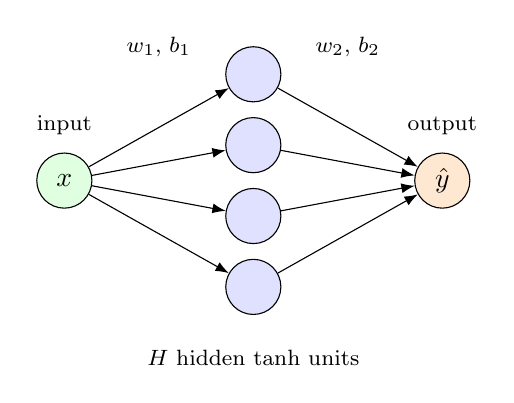
\begin{tikzpicture}[>=Latex, unit/.style={circle,draw,minimum size=7mm,inner sep=0pt}]
  \node[unit,fill=green!12] (x) at (0,-2.25) {$x$};
  \foreach \i in {1,...,4} { \node[unit,fill=blue!12] (h\i) at (2.4,-\i*0.9) {}; }
  \node[unit,fill=orange!18] (y) at (4.8,-2.25) {$\yhat$};
  \foreach \i in {1,...,4} { \draw[->] (x) -- (h\i); \draw[->] (h\i) -- (y); }
  \node[above=1mm of x] {\footnotesize input};
  \node[above=1mm of y] {\footnotesize output};
  \node at (2.4,-4.5) {\footnotesize $H$ hidden $\tanh$ units};
  \node at (1.2,-0.55) {\footnotesize $\wvec_1,\,b_1$};
  \node at (3.6,-0.55) {\footnotesize $\wvec_2,\,b_2$};
\end{tikzpicture}
\caption{The student network of \eqref{eq:net}: one scalar input, $H$ hidden
$\tanh$ units, one scalar output. All weights and biases are the decision
variables of the NLP.}
\label{fig:net}
\end{figure}

\subsection{The desired constrained problem}
The modelling goal is to fit the data while guaranteeing that the network does not
react too fast to input changes. Writing this requirement directly, the ideal
training problem is
\begin{mini}
{\wvec}{f(\wvec)}{\label{eq:idealnlp}}{}
\addConstraint{\displaystyle\sup_{x\neq x'}
\frac{|\yhat(x;\wvec)-\yhat(x';\wvec)|}{|x-x'|}}{\le\Lmax}
\addConstraint{\norm{\wvec}_2^2}{\le\Bmax^2.}
\end{mini}
Here $f(\wvec)$ is the training error \eqref{eq:mse}; the first constraint is the true
input Lipschitz requirement with bound $\Lmax$; and the second is the parameter-norm
ball of radius $\Bmax$. The supremum is not directly convenient for a numerical NLP
solver, so it is replaced next by a conservative, computable sufficient condition.

\subsection{Derivation of the tractable certificate}
For fixed weights $\wvec$, denote the true input Lipschitz constant of the network by
$\Lip(\wvec)$. Because the network in \eqref{eq:net} is differentiable,
\begin{equation}
\Lip(\wvec)=\sup_x\left|\frac{\mathrm d\yhat(x;\wvec)}{\mathrm dx}\right|.
\label{eq:truelip}
\end{equation}
Differentiating,
\begin{equation}
\frac{\mathrm d\yhat}{\mathrm dx}
=\wvec_2^\top\,\mathrm{diag}\!\bigl(1-\tanh^2(\wvec_1 x+b_1)\bigr)\,\wvec_1 .
\label{eq:deriv}
\end{equation}
Each diagonal entry lies in $(0,1]$, so the diagonal matrix has operator norm at
most one, and Cauchy--Schwarz gives
\begin{equation}
\Lip(\wvec)\le\norm{\wvec_1}_2\,\norm{\wvec_2}_2=:\Uc .
\label{eq:cert}
\end{equation}
The certificate $\Uc$ is computable and is an \emph{upper bound}: it is not equal to
the true Lipschitz constant in general, and $\Uc\le\Lmax$ is a conservative
sufficient condition for the true requirement
$\Lip(\wvec)\le\Lmax$. I impose it in the squared form
\begin{equation}
\norm{\wvec_1}_2^2\,\norm{\wvec_2}_2^2\le\Lmax^2,
\label{eq:c1}
\end{equation}
a degree-four (biquadratic) polynomial in the weights: smooth, but nonconvex.
Replacing the true Lipschitz constraint by \eqref{eq:c1} gives the tractable NLP
actually solved,
\begin{mini}
{\wvec}{f(\wvec)}{\label{eq:nlp}}{}
\addConstraint{\norm{\wvec_1}_2^2\,\norm{\wvec_2}_2^2}{\le\Lmax^2}
\addConstraint{\norm{\wvec}_2^2}{\le\Bmax^2.}
\end{mini}

\section{Numerical Optimization}\label{sec:numopt}
\subsection{Hard-constrained solution}
The objective and constraints of \eqref{eq:nlp} are assembled symbolically in
CasADi~\cite{casadi}, which supplies exact first and second derivatives, and the
smooth nonconvex program is solved by the interior-point method IPOPT~\cite{ipopt}.
The hard solves run to a KKT tolerance of $10^{-8}$; here feasibility means the
constraints are satisfied to solver tolerance, not that a global optimum has been
certified.

\subsection{Soft-penalty baseline and protocol}
The baselines replace the hard constraints by penalties. \emph{Plain Adam}~\cite{adam}
minimizes only the MSE; \emph{AdamW}~\cite{adamw} adds decoupled weight decay with
coefficient $\wdcoef$, a soft stand-in for the norm ball; \emph{penalty-Adam} adds
both requirements as a hinge penalty
\begin{equation}
\min_{\wvec} f(\wvec)+\rho\bigl[\max(0,\norm{\wvec_1}_2^2\norm{\wvec_2}_2^2-\Lmax^2)
+\max(0,\norm{\wvec}_2^2-\Bmax^2)\bigr],
\label{eq:penalty}
\end{equation}
minimized with Adam, where $\rho\ge0$: too small and the requirements are violated,
too large and the nonsmooth term stiffens the first-order optimization.

\emph{Stopping and initialization.} Every gradient run stops at a loss plateau
(successive change below $10^{-9}$) with a cap of \num{40000} iterations; reaching
the cap is reported as non-converged. The hard IPOPT solves use tolerance $10^{-8}$,
and the exact-penalty sweep of Section~\ref{sec:synth} uses IPOPT tolerance
$10^{-10}$ with acceptable tolerance $10^{-9}$. Within any matched comparison all
methods start from the same initialization; the initialization changes with the seed
across repeated trials.

\section{Case Studies}\label{sec:cases}
Two regression tasks illustrate the formulation: a synthetic teacher--student
problem and a simulated damped pendulum.

\subsection{Synthetic case study}\label{sec:synth}
The synthetic tasks draw inputs $x_i\sim\mathrm{Uniform}[-3,3]$ and targets
$y_i=y_T(x_i;\wvec^\star)+\varepsilon_i$ with $\varepsilon_i\sim\mathcal N(0,\sigma^2)$,
where the teacher $y_T$ is a seeded one-hidden-layer $\tanh$ network of six units and
the student has $H$ units. Changing the seed changes the teacher weights, the input
sample, the noise and the initialization together, so a set of seeds gives
independently seeded teacher--student trials rather than repeated noise on one fixed
target.

\subsubsection{Optimizer diagnostic}
Fig.~\ref{fig:conv} plots, against iteration, a running-minimum optimality diagnostic
for the two solver families. For IPOPT on the hard-constrained NLP it is the running
minimum up to iteration $k$ of $\max(\mathrm{inf\_pr},\mathrm{inf\_du})$, IPOPT's
primal and dual infeasibility measures; for plain Adam it is the running minimum of
$\norm{\nabla f(\wvec_j)}_\infty$, the infinity norm of the plain-Adam objective
gradient at iteration $j$. These are different,
solver-specific quantities, and plain Adam here minimizes only the MSE rather than
solving the hard-constrained NLP, so their absolute vertical values are not directly
comparable; the plot shows only the qualitative evolution of each method's own
diagnostic.

\begin{figure}[t]
\centering
\includegraphics[width=0.86\columnwidth]{figures/fig_convergence.png}
\caption{Running minimum of solver-specific optimality diagnostics versus iteration.
IPOPT shows $\max(\mathrm{inf\_pr},\mathrm{inf\_du})$ for the hard-constrained solve;
plain Adam shows the infinity norm of its gradient. The quantities are different and
are compared only qualitatively.}
\label{fig:conv}
\end{figure}

\subsubsection{Certificate control}
Can a method \emph{set} the certificate rather than merely influence it? I fit the
synthetic target with $H=8$, $\Lmax=4$, $\Bmax=6$, on $60$ training and $40$ test
points, at two noise levels $\sigma\in\{0.1,0.3\}$, over $15$ independently seeded
trials. Table~\ref{tab:sens} reports the certificate
$\Uc=\norm{\wvec_1}\norm{\wvec_2}$ of the hard solve and of the Adam baselines.
IPOPT satisfies $\Uc\le4$ in every trial, with the certificate active near the
boundary to solver tolerance (median $4.00$ at both noise levels, zero violations).
Plain Adam does not control it, and worsens with noise; AdamW improves matters but
still violates the bound in a third of the low-noise trials and in all high-noise
trials. Its weight-decay coefficient $\wdcoef$ was chosen on a pilot seed (seed $0$)
by test error, to give the baseline a strong setting; this is a transparent modelling
choice, not a validation-tuned result.

\begin{table}[t]
\caption{Certificate $\Uc=\norm{\wvec_1}\norm{\wvec_2}$ over $15$ independently
seeded trials (median $[\min,\max]$) and the number that violate $\Lmax=4$. IPOPT
stays on the bound to solver tolerance; the Adam baselines are uncontrolled and
worsen with noise.}
\label{tab:sens}
\centering\setlength{\tabcolsep}{4pt}\footnotesize
\begin{tabular}{@{}llcc@{}}
\toprule
$\sigma$ & Method & $\Uc$ (median $[\min,\max]$) & Viol.\ of $4$\\
\midrule
$0.1$ & IPOPT (hard)                 & $4.00\ [4.00,\ 4.00]$   & $0/15$\\
$0.1$ & plain Adam                   & $5.83\ [1.27,\ 24.0]$   & $10/15$\\
$0.1$ & AdamW ($\wdcoef=0.01$)       & $3.19\ [0.91,\ 11.1]$   & $5/15$\\
$0.3$ & IPOPT (hard)                 & $4.00\ [4.00,\ 4.00]$   & $0/15$\\
$0.3$ & plain Adam                   & $63.4\ [6.7,\ 399]$     & $15/15$\\
$0.3$ & AdamW ($\wdcoef=10^{-4}$)    & $44.2\ [6.7,\ 153]$     & $15/15$\\
\bottomrule
\end{tabular}
\end{table}

\subsubsection{Exact-penalty analysis}
This experiment specializes the soft penalty \eqref{eq:penalty} to the single
certificate constraint and solves it to convergence with an IPOPT epigraph
reformulation, which isolates the formulation effect from a fixed-budget Adam run. On
a fixed teacher (seed $2$, $\sigma=0.2$, $40$ training / $40$ validation / $40$ test
points, only the certificate constraint included) the hard reference sits on the
bound at $\Uc=4.00$ with KKT multiplier $\lambda^\star=\num{1.6e-4}$, training MSE
$0.033$ and test MSE $0.066$. Fig.~\ref{fig:penalty} shows a feasibility transition
close to this multiplier: below $\lambda^\star$ the certificate exceeds $\Lmax$
(about $7.9,6.6,5.8$), and the first sampled value above $\lambda^\star$,
$\rho=\num{1.7e-4}$, already sits on the bound, as do the subsequent sampled values.
Because the problem is nonconvex, exact-penalty theory~\cite{nocedalwright}
guarantees only local exactness once $\rho$ exceeds the relevant multiplier; I read
the plot as a feasibility transition near the hard solution's multiplier, not as
proof that every larger $\rho$ returns the identical parameter vector.

\begin{figure}[t]
\centering
\includegraphics[width=0.9\columnwidth]{figures/fig_exact_penalty.png}
\caption{Converged exact-penalty sweep for the certificate constraint. The
certified bound $\Uc$ of the converged epigraph solve exceeds $\Lmax=4$ for
$\rho<\lambda^\star$; the first sampled value above $\lambda^\star$, and subsequent
sampled values, lie on the boundary, matching the hard-constrained IPOPT reference.}
\label{fig:penalty}
\end{figure}

\subsubsection{Width scaling}
Bigger networks do not fit this target better, but the hard solve costs steeply more.
The width experiment uses $\sigma=0.05$, seed $0$, $\Lmax=4$, $\Bmax=6$, and $60$
training / $40$ test points, and compares IPOPT against penalty-Adam on the same two
requirements. Growing $H$ from $4$ to $256$ ($n$ from $13$ to $769$;
Fig.~\ref{fig:scaling}) leaves the test error near $0.003$ for both methods, so the
added capacity buys no accuracy. IPOPT satisfies the certificate bound in every run,
with the certificate generally near the boundary ($\Uc\approx4.00$); its solve time
rises from about \SI{0.14}{\second} to about \SI{453}{\second}, while penalty-Adam
takes about \SI{13.2}{\second}. On this implementation and the measured range
($n\ge49$) the interior-point time grows empirically about as $n^{2.3}$; this is a
fit to the measured points of one run, not a universal complexity law, and wall-clock
timings are not expected to reproduce exactly. The mechanism is that each
interior-point iteration solves a KKT linear system whose cost grows with the number
of decision variables.

\begin{figure}[t]
\centering
\includegraphics[width=\columnwidth]{figures/fig_scaling.png}
\caption{Width scaling from $H=4$ to $256$: IPOPT cost grows steeply, while test MSE remains nearly flat for both methods.}
\label{fig:scaling}
\end{figure}

\subsection{Simulated damped-pendulum case study}\label{sec:pend}
As a small dynamics-flavoured task I fit the \emph{simulated} free response of a
linearized damped pendulum,
\begin{equation}
\begin{aligned}
\theta(t)
&=\theta_0 e^{-\zeta\omega t}
\left[\cos(\omega_d t)
+\frac{\zeta\omega}{\omega_d}\sin(\omega_d t)\right],\\
\omega_d
&=\omega\sqrt{1-\zeta^2}.
\end{aligned}
\label{eq:pend}
\end{equation}
with $\theta_0=\SI{1}{\radian}$, $\omega=\SI{2}{\radian\per\second}$, $\zeta=0.15$
and $t\in[0,\SI{6}{\second}]$; this is a simulated response, not a measurement of a
physical rig. Observations are $t_i\sim\mathrm{Uniform}[0,6]$,
$y_i=\theta(t_i)+\varepsilon_i$, $\varepsilon_i\sim\mathcal N(0,0.15^2)$, split into
$60$ training / $60$ validation / $60$ test points; $\rho$ for the soft method is
chosen on the validation split and the reported error is on the test split. The
bound $\Lmax=\SI{4}{\radian\per\second}$ is a fixed demonstration requirement on the
learned model's rate $|\mathrm d\hat\theta/\mathrm dt|$, not a value inferred from the
physics.

Table~\ref{tab:pend} and Fig.~\ref{fig:pendulum} compare the hard solve with matched
penalty-Adam. IPOPT converges in $103$ iterations (\SI{0.09}{\second}), satisfying
both constraints ($\Uc=4.00$, $\norm{\wvec}=6.00$) at test MSE $0.0232$.
penalty-Adam at $\rho=0.01$ reaches the \num{40000}-iteration cap without meeting its
convergence criterion; its final iterate is numerically feasible ($\Uc=3.93$,
$\norm{\wvec}=5.94$) at test MSE $0.0243$. The test errors are close: the difference
is direct constraint enforcement and reliable convergence, not predictive accuracy.

\begin{table}[t]
\caption{Pendulum: the hard solve versus matched penalty-Adam. Only IPOPT converges;
penalty-Adam reaches the iteration cap with a numerically feasible but non-converged
iterate.}
\label{tab:pend}
\centering\setlength{\tabcolsep}{6pt}\footnotesize
\begin{tabular}{@{}lcccc@{}}
\toprule
Method & $\Uc$ & $\norm{\wvec}$ & Test MSE & Converged?\\
\midrule
IPOPT (hard)        & $4.00$ & $6.00$ & $0.0232$ & yes ($10^{-8}$)\\
penalty-Adam (soft) & $3.93$ & $5.94$ & $0.0243$ & no (cap)\\
\bottomrule
\end{tabular}
\end{table}

\begin{figure}[t]
\centering
\includegraphics[width=0.9\columnwidth]{figures/fig_pendulum.png}
\caption{Damped-pendulum fits: noisy samples (grey), the simulated true response
(dashed) and the two matched models. IPOPT certifies
$|\mathrm d\hat\theta/\mathrm dt|\le\SI{4}{\radian\per\second}$; penalty-Adam fits
similarly but did not converge.}
\label{fig:pendulum}
\end{figure}

\section{Extension to Deeper Neural Networks}\label{sec:deep}
The one-hidden-layer exposition used vectors because the input and output are scalar.
A network with $D$ hidden layers of width $H$ is defined by
\begin{equation}
\begin{aligned}
h_1&=\tanh(W_1 x+b_1),\\
h_l&=\tanh(W_l h_{l-1}+b_l),\quad l=2,\ldots,D,\\
\yhat(x;\wvec)&=W_{D+1}h_D+b_{D+1},
\end{aligned}
\label{eq:deepnet}
\end{equation}
with $W_1\in\mathbb{R}^{H\times1}$ a column, $W_l\in\mathbb{R}^{H\times H}$ genuine
square matrices for $l=2,\ldots,D$, and $W_{D+1}\in\mathbb{R}^{1\times H}$ a row.
Although the overall network maps $\mathbb{R}$ to $\mathbb{R}$, every hidden state
$h_l$ lies in $\mathbb{R}^H$, so the internal maps $W_l:\mathbb{R}^H\to\mathbb{R}^H$
are genuinely multidimensional. Their relevant size is the spectral norm
\begin{equation}
\norm{W}_2:=\sup_{v\neq0}\frac{\norm{Wv}_2}{\norm{v}_2},
\label{eq:spectral}
\end{equation}
the induced Euclidean norm, which is the Lipschitz constant of the affine map
$z\mapsto Wz+b$. Since $\tanh$ is $1$-Lipschitz and Lipschitz constants multiply under
composition, the natural multilayer bound is the product of the layer spectral norms,
\begin{equation}
\Lip(\wvec)
\le\prod_{l=1}^{D+1}\norm{W_l}_2\le\prod_{l=1}^{D+1}\norm{W_l}_F=:U_F(\wvec).
\label{eq:deepcert}
\end{equation}
The second inequality uses the Frobenius norm
\begin{equation}
\norm{W}_F^2=\sum_{i,j}W_{ij}^2,
\label{eq:frob}
\end{equation}
and $\norm{W}_2\le\norm{W}_F$, so the Frobenius-product certificate $U_F(\wvec)$ is a
conservative upper bound on the spectral-product one. The implementation constrains
$U_F(\wvec)$ because its squared form
\begin{equation}
\prod_{l=1}^{D+1}\norm{W_l}_F^2\le\Lmax^2
\label{eq:frobcon}
\end{equation}
is a smooth polynomial in the weights, convenient for the CasADi/IPOPT formulation; the
trade-off is a potentially looser certificate than the spectral-norm product. For the
scalar-input, scalar-output layers $W_1\in\mathbb{R}^{H\times1}$ and
$W_{D+1}\in\mathbb{R}^{1\times H}$ the spectral, Frobenius and Euclidean norms coincide;
the distinction matters only for the internal $H\times H$ matrices.

The depth experiment stacks $1$ to $6$ hidden layers of width $8$ ($n$ from $25$ to
$385$), with $\sigma=0.05$, seed $0$, $\Lmax=4$, $\Bmax=6$ and $60$ training / $40$
test points. IPOPT satisfies the Frobenius-product certificate $U_F(\wvec)$ to solver
tolerance at every depth, whereas unconstrained Adam's $U_F(\wvec)$ grows from about
$1.75$ at one layer to about $2.5\times10^{5}$ at six (Fig.~\ref{fig:depth}). Test
errors stay near $0.003$, so depth buys no accuracy, while the solve time grows from
about \SI{0.38}{\second} to about \SI{57}{\second} for IPOPT and from about
\SI{0.27}{\second} to about \SI{21}{\second} for penalty-Adam (Table~\ref{tab:depth},
Fig.~\ref{fig:depthcost}). IPOPT converged for every configuration in the tested
range of one to six hidden layers; the limit is expense, not failure.

\begin{figure}[t]
\centering
\includegraphics[width=0.86\columnwidth]{figures/fig_depth.png}
\caption{Frobenius-product certificate $U_F(\wvec)=\prod_l\norm{W_l}_F$ versus depth
(log scale). The constraint keeps it near $\Lmax=4$ while satisfying the bound at
every depth; unconstrained Adam grows past $2.5\times10^{5}$ at six hidden layers.}
\label{fig:depth}
\end{figure}

\begin{table}[t]
\caption{Depth study (width $8$ per layer, $1$--$6$ hidden layers, $n=25$ to $385$):
matched IPOPT vs penalty-Adam. Depth buys no accuracy; IPOPT converges at every
depth but its cost grows steeply.}
\label{tab:depth}
\centering\setlength{\tabcolsep}{5pt}\footnotesize
\begin{tabular}{@{}cccccc@{}}
\toprule
& & \multicolumn{2}{c}{IPOPT (hard)} & \multicolumn{2}{c}{penalty-Adam}\\
\cmidrule(lr){3-4}\cmidrule(lr){5-6}
Depth & $n$ & Test & Time [\si{\second}] & Test & Time [\si{\second}]\\
\midrule
1 & 25  & 0.0031 & 0.38  & 0.0029 & 0.27\\
2 & 97  & 0.0033 & 1.33  & 0.0029 & 0.70\\
3 & 169 & 0.0031 & 7.81  & 0.0030 & 3.19\\
4 & 241 & 0.0031 & 15.59 & 0.0028 & 7.61\\
5 & 313 & 0.0030 & 31.15 & 0.0027 & 6.20\\
6 & 385 & 0.0032 & 57.44 & 0.0028 & 21.21\\
\bottomrule
\end{tabular}
\end{table}

\begin{figure}[t]
\centering
\includegraphics[width=\columnwidth]{figures/fig_depth_cost.png}
\caption{Depth scaling over $1$--$6$ hidden layers: solve time increases, especially for IPOPT, while test MSE remains nearly flat.}
\label{fig:depthcost}
\end{figure}

\section{Conclusion and Critical Discussion}
The true Lipschitz requirement is replaced conservatively by the computable
certificate $\Uc$. When the resulting NLP is solved with IPOPT through CasADi, the
network satisfies the certificate bound and norm ball to solver tolerance without a
penalty weight. A soft-penalty Adam baseline must instead choose $\rho$ and can fail
to converge within a fixed iteration budget. Predictive errors are similar across the
tested examples, and neither width nor depth improves accuracy on this small target;
what grows is the cost of the hard solve, steeply with the number of weights. The
approach is therefore suited to small constrained training problems where a certified
requirement matters, rather than to large-scale neural-network training. Natural
extensions are stochastic or mini-batch constraint handling for larger data, tighter
spectral-norm certificates in place of the Frobenius product, and structure-exploiting
KKT solvers to raise the size at which the hard solve stays affordable.

\begin{thebibliography}{9}
\bibitem{casadi} J.~A.~E. Andersson, J.~Gillis, G.~Horn, J.~B. Rawlings, and
M.~Diehl, ``CasADi: a software framework for nonlinear optimization and optimal
control,'' \emph{Math. Program. Comput.}, vol.~11, no.~1, pp.~1--36, 2019.
\bibitem{ipopt} A.~W\"achter and L.~T. Biegler, ``On the implementation of an
interior-point filter line-search algorithm for large-scale nonlinear
programming,'' \emph{Math. Program.}, vol.~106, no.~1, pp.~25--57, 2006.
\bibitem{adam} D.~P. Kingma and J.~Ba, ``Adam: a method for stochastic
optimization,'' in \emph{Int. Conf. Learn. Representations (ICLR)}, 2015.
\bibitem{adamw} I.~Loshchilov and F.~Hutter, ``Decoupled weight decay
regularization,'' in \emph{Int. Conf. Learn. Representations (ICLR)}, 2019.
\bibitem{gouk} H.~Gouk, E.~Frank, B.~Pfahringer, and M.~J. Cree, ``Regularisation
of neural networks by enforcing Lipschitz continuity,'' \emph{Mach. Learn.},
vol.~110, no.~2, pp.~393--416, 2021.
\bibitem{miyato} T.~Miyato, T.~Kataoka, M.~Koyama, and Y.~Yoshida, ``Spectral
normalization for generative adversarial networks,'' in \emph{ICLR}, 2018.
\bibitem{nocedalwright} J.~Nocedal and S.~J. Wright, \emph{Numerical
Optimization}, 2nd ed. New York: Springer, 2006.
\end{thebibliography}

\end{document}
